\chapter{Seamless modeling of retarded vdW interactions}\label{chap:casimir}

{\sffamily\mathversion{sans} This chapter briefly discusses the extension of the MBD method to distances at which the finite speed of light cannot be neglected, resulting in the so-called retarded vdW (Casimir) interactions.
Previously, microscopic models of vdW interactions such as MBD were restricted to the non-retarded regime, whereas the macroscopic continuous models used for description of Casimir interactions could not be used at short distances and must have been parametrized from experimental data.
Here, we show that these two descriptions can be unified within a single framework, which then enables seamless calculation of vdW energies both at the non-retarded and retarded (Casimir) regimes.
This unification also extends the applicability of the new developments in Chapter~\ref{chap:polarizability}, because any improvements in a model of material response can be directly used in the study of Casimir physics.
The results discussed in this chapter have been published in \citep*{VenkataramPRL17}.
The Maxwell-equation scattering calculations were done by Prashanth Venkataram, the DFT and polarizability screening calculations by myself, and the unified theoretical framework is a result of joint work.
}\vspace{1em}

The ACFD formula and hence the MBD correlation energy in~\eqref{eq:mbd-rpa} originate from the nonrelativistic quantum mechanics, which assumes that the electromagnetic forces in the form of the Coulomb law acts instantly over any distance.
This limits the applicability of MBD to systems that are separated by less than hundreds of angstroms, at which point the time it takes for light to travel between the interacting objects becomes comparable to the frequency of the electronic oscillations that drive the vdW interactions.
(The speed of light, $c$, in atomic units is approximately 137, the inverse of the fine-structure constant.)
The well-known effect of this retardation of the electromagnetic force is the asymptotic $1/R^7$ attraction that replaces the nonrelativistic $1/R^6$ power law.

The extension of MBD to account for this retardation consists of two steps.
First, the instantaneous dipole operator (eq.~\ref{eq:dipole-op}) is replaced with its frequency-dependent retarded version, which is proportional to the Green's function, $\boldsymbol G_0$, of the electric field,
\begin{equation}
  \tilde{\mathbf T}(\mathbf R,u)=\frac{4\pi u^2}{c^2}\boldsymbol G_0=\big(\boldsymbol\nabla\otimes\boldsymbol\nabla'-\tfrac{u^2}{c^2}\mathbf I\big)\mathrm e^{-|\mathbf r-\mathbf r'|u/c}v(|\mathbf r-\mathbf r'|)\Big|_{\substack{\mathbf r=\mathbf R\\\mathbf r'=\mathbf 0}}
  \label{eq:green-maxwell}
\end{equation}
This substitution prevents one to perform the analytic integration over frequencies analytically (see eq.~\ref{eq:mbd-rpa}), but otherwise it is a straightforward modification of the MBD method.

The second step is necessary only because of the kind of systems that we want to study.
The prototypical systems studied in the context of Casimir interactions consist of small microscopic bodies such as molecules, and macroscopic objects with nontrivial shapes or surface gratings~\cite{RodriguezNP11,WoodsRMP16}.
The latter are typically large enough that microscopic description of individual atoms in them is unnecessary and, furthermore, such large atomic calculations would be unfeasible.
As an alternative, efficient approaches solve directly the continuous Maxwell equations either with scattering or finite-differencing methods~\cite{RodriguezPRA07,RahiPRD09}.
This raises the issue of connecting the continuous and microscopic descriptions.
It turns out that such a connection is naturally enabled by the form of the MBD expression for the interaction energy.
Consider the MBD interaction energy of two bodies, $A$ and $B$,
\begin{equation}
\begin{aligned}
E_\text{int}&=E_{AB}-E_{A}-E_{B} \\
&=\frac1{2\pi}\int_0^\infty\mathrm du\operatorname{Tr}\big(\ln(1+(\boldsymbol\alpha_A+\boldsymbol\alpha_B)\tilde{\mathbf T})-\ln(1+\boldsymbol\alpha_A\tilde{\mathbf T})-\ln(1+\boldsymbol\alpha_B\tilde{\mathbf T})\big) \\
&=\frac1{2\pi}\int_0^\infty\mathrm du\operatorname{Tr}\big(\ln((1+\boldsymbol\alpha_A\tilde{\mathbf T}+\boldsymbol\alpha_B\tilde{\mathbf T})(1+\boldsymbol\alpha_A\tilde{\mathbf T})^{-1}(1+\boldsymbol\alpha_B\tilde{\mathbf T})^{-1})\big) \\
&=\frac1{2\pi}\int_0^\infty\mathrm du\operatorname{Tr}\big(\ln((1+\boldsymbol\alpha_B\tilde{\mathbf T}(1+\boldsymbol\alpha_A\tilde{\mathbf T})^{-1})(1+\boldsymbol\alpha_B\tilde{\mathbf T})^{-1})\big) \\
&\equiv\frac1{2\pi}\int_0^\infty\mathrm du\operatorname{Tr}\big(\ln((1+\boldsymbol\alpha_B\tilde{\mathbf T}_A)(1+\boldsymbol\alpha_B\tilde{\mathbf T})^{-1})\big) \\
&=\frac1{2\pi}\int_0^\infty\mathrm du\operatorname{Tr}\big(\ln(1+\boldsymbol\alpha_B\tilde{\mathbf T}_A)-\ln(1+\boldsymbol\alpha_B\tilde{\mathbf T})\big) \\
&=E_B(\tilde{\mathbf T}_A)-E_B(\tilde{\mathbf T})
\end{aligned}
\label{eq:casimir-mbd}
\end{equation}
Here, we defined $\tilde{\mathbf T}_A=\tilde{\mathbf T}(1+\boldsymbol\alpha_A\tilde{\mathbf T})^{-1}$, which is the retarded dipole operator screened by the electromagnetic response of the body $A$, and the interaction energy between $A$ and $B$ was recast as the difference in the total energy of $B$ calculated with the bare and screened dipole operators.
The definition of $\tilde{\mathbf T}_A$ has the form of a Dyson-like equation analogous to that for the interacting nonlocal polarizability, which points to two equivalent points of view on the ground-state system of bodies of matter interacting via the electromagnetic force---one as fluctuating polarizations of the electronic density propagated (in the Green's function sense) by the electromagnetic field, the other as fluctuations in the electromagnetic field propagated by the electronic response of the matter.

\begin{figure}[t]
\centering
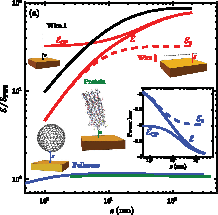
\includegraphics[width=10cm]{media/casimir.pdf}
\caption{\textbf{Retardation effects in vdW interactions.}
Interaction energies of a perpendicular (black) and parallel (red) carbyne wire, fullerene C$_{500}$, and a protein with a golden surface calculated with different models are plotted relative to the prediction of a pairwise approximation as a function of the vertical distance, $z$.
$\mathcal{E}$ is the full retarded MBD method (eq.~\ref{eq:casimir-mbd}), $\mathcal{E}_0$ is the nonrelativistic approximation ($c\rightarrow\infty$ in~\eqref{eq:green-maxwell}), and $\mathcal E_\text{CP}$ is the so-called ``Casimir--Polder approximation'' which approximates the whole microscopic object with a single point.
The inset shows the local power-law asymptote for the plate--fullerene system.
}\label{fig:casimir}
\end{figure}

Using the formulation in~\eqref{eq:casimir-mbd}, the MBD interaction energy of a macroscopic body (which can be also a collection of macroscopic bodies) and a set of microscopic objects can be calculated in the following way.
First, one obtains the Green's function of the electric field in the presence of the macroscopic body by an efficient continuous macroscopic method.
Second, the screened retarded dipole operator is calculated from the Green's function using~\eqref{eq:green-maxwell}.
Third, the vdW interaction energy is calculated using the regular MBD method with the screened and bare dipole operators according to~\eqref{eq:casimir-mbd}.
Figure~\ref{fig:casimir} illustrates the effects of the retardation on the interactions of several prototypical systems with a golden plate.
The full retarded MBD interaction energy calculated with~\ref{eq:casimir-mbd} transitions between the nonrelativistic approximation (the regular MBD), which becomes exact at short distances, and the relativistic Casimir--Polder approximation, which models the microscopic objects as point objects, and becomes exact at large separations.
In this regard, this unified framework represents a new seamless approach to multi-scale modeling that enables accurate description of intermolecular interactions at a range spanning several orders of magnitude.
